\chapter{Background} \label{chap:background}

\section{Organic Semiconductors}

%When atoms bond together, molecular orbital are defined by the linear combination of atomic orbitals, however the symmetry shown on some complex structures are not explained by a simple linear combination, instead hybrid atomic orbitals are formed. This mathematical process is called \textbf{hybridization}.
Unlike inorganic semiconductors, organic semiconductors are lightweight, easy to chemical tune, mechanical flexible, and possess low-cost and low-temperature processing. All of these characteristics increased the attention to this type of materials in the field of organic electronics. 

%\subsection{Conjugated polymers}
%\subsection{Small molecules}

\subsection{Electronic Structure} 

Organic semiconductors are $\pi$-conjugated molecules that comprise mostly carbon and hydrogen atoms, with alternating multiple (sp$^{3}$, sp$^{2}$ hybridization) and single (sp hybrization) bonds. This configuration exhibit $p$ orbitals with delocalized electrons, charge transport among the length of these polymers is caused by this resonance structure. Based on the size of the conjugated system, organic semiconductors can be divided into conjugated polymers and small molecules.

\subsubsection{Conjugated polymers}
%Semiconducting properties of conjugated polymers built by alternating electron donor and acceptor moieties \cite{mattElectronicStructureMorphology2021}, 
%Since inorganic semiconductors' band models does not take into consideration the Coulomb and exchange electron-electron interaction, which play a major role in organic semiconductors, it is necessary to add new theoretical approaches. On one hand, the transport properties are better described in terms of a hopping mechanism and the optoelectronic properties are better described by the molecular orbital picture \cite{alcacerElectronicStructureOrganic2018}. Since the device under study in this work is a transistor and their transport properties in aqueous and quasi-solid environments, the theoretical approach used will be the hopping mechanism.

%Transport properties depend on the details of the band structure, namely the density of states and the band widths

\subsubsection{Small Molecules}
%Unlike conjugated polymers, the chain size of small molecules have the advantage of being ordered and its synthesis allow to obtain high purity material.

\subsection{Molecular Doping} \label{subsec:moldop}
The basic principles are similar than in inorganic materials, "where electron donors or acceptors are added and generate additional mobile charge carriers", as shown in Figure \ref{fig:doping}. While n-type dopants donate electrons to the lowest unoccupied molecular orbital (LUMO) states, the "p-type dopants extract electrons from the highest occupied molecular orbital (HOMO) states", hence creates holes \cite{lussemDopingOrganicSemiconductors2013}. In other words, the Fermi level E$_{F}$ of the polymer will shift towards the LUMO (or HOMO) level when n-type (or p-type) doping. Shift that can be measured by spectroscopy techniques such as Ultraviolet Photoelectron Spectroscopy (UPS) at room temperature (RT) \cite{tietzeFermiLevelShift2012}, limited to the penetration depth of the incoming electron.

\begin{figure}
  \centering
  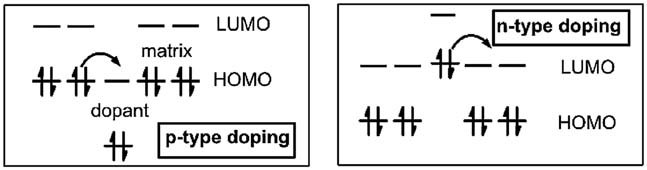
\includegraphics[width=12cm]{Images/doping.jpg}
  \caption{Schemes for p-type (left) and n-type (right) doping processes. Extracted from reference \cite{lussemDopingOrganicSemiconductors2013}.}
  \label{fig:doping}
\end{figure}

%% This specifics introduces to our graph
The use of small molecules is commonly reported as dopants for organic materials. Some strong acceptor (or electron-defficient) molecules that are widely used are 2,3,5,6 tetrafluoro-7,7,8,8-tetracyanoquinodimethane (F$_{4}$TCNQ) or 1,3,4,5,7,8 hexafluoro-7,7,8,8-tetracyanonaphthoquinodimethane (F$_{6}$TCNQ), which also take part in this work. The latter exhibits a higher electronic affinity (-5.3 eV) or deep HOMO than F$_{4}$TCNQ (-5.2eV) meaning that it can abstract more electrons, specially to polymers with low ionization potential (less than 5eV) or shallow LUMO, \cite{kieferDoubleDopingConjugated2019}, as it is the case of p(g3T2-T) acting as donor.

Among the different methods to molecular doped a conjugated polymer, Jacobs et al. compared a solution-mixed and solution sequential doping of P3HT (a thiophene-based polymer) doped with F$_{4}$TCNQ, both straightforward and easy methods for doping \cite{jacobsComparisonSolutionmixedSequentially2016}. In this work it was demonstrated that solution-mixed films are considerably rougher than solution-sequential films, affecting negatively to its conductivity. The fact that solution-sequential doped films allows better homogeneity, make it also more compatible with microstructuring processes such as photolithography. At the expense of having less control over the doping levels compared to solution-mixed films \cite{tanOrganicMixedIonic2022}.


%\subsubsection{Techniques for doping conjugated polymers}

%\subsubsection{Measuring techniques to characterize doping}

\section{Organic Mixed Ionic/Electronic Conductors (OMIECs)} \label{sec:omiecs}

Organic Mixed Ionic/Electronic conductors are organic semiconductors that allow the conduction of electrons (or holes) and ions, the latter set them apart from other organic semiconductors. %Organic semiconductors 
Commonly structured with polar sidechains, they have been identified as a promising class of materials for the field of bioelectronics
%These materials, also called organic mixed ionic/electronic conductors (OMIECs), can exchange ions with aqueous electrolytes when electronic charge carriers are injected, transported, and stored in the bulk of the material
\cite{giovannittiEnergeticControlRedoxActive2020}. Initially investigated for batteries and super capacitors \cite{snookConductingpolymerbasedSupercapacitorDevices2011}
\cite{liangOrganicElectrodeMaterials2012}, where the induction of charges in a semiconducting polymer was the main objective. OMIECs has rapidly grown to include other applications, among them, our focus: OECTs.\\

Paulsen et al. classified OMIECs into six different categories according to whether they \textit{``intrinsically contain ionic charge''} (I, III, V) or not (II, IV, VI), the latter "contain polar moieties that can solvate ions". Another distinction among the categories is whether the conjugated system comprises a single material (homogeneous, type V and VII) or two-component, more complex systems or block co-polymers materials (heterogeneous, type I, II, III, IV)\cite{paulsenOrganicMixedIonic2020}, an schematic representation is shown in Figure \ref{fig:omiectypes}. 

%Electronic charges accumulated on the conjugated polymer backbone result in secondary property changes in electrochemical potential and electronic conductivity \cite{tanOrganicMixedIonic2022}. 

% PEDOT:PSS Heterogeneous, blends or complexed systems OMIEC. Conjugated polymer/electrolyte blends. Contains ions chemically linked ot an insulating or conjugated component
% p(g3T2-T) Homogeneous, single-component systems OMIEC. Conjugated polymer electrolytes. Ions introduced as free species upon material casting or device operation

%change caption of figure
\begin{figure}
  \centering
  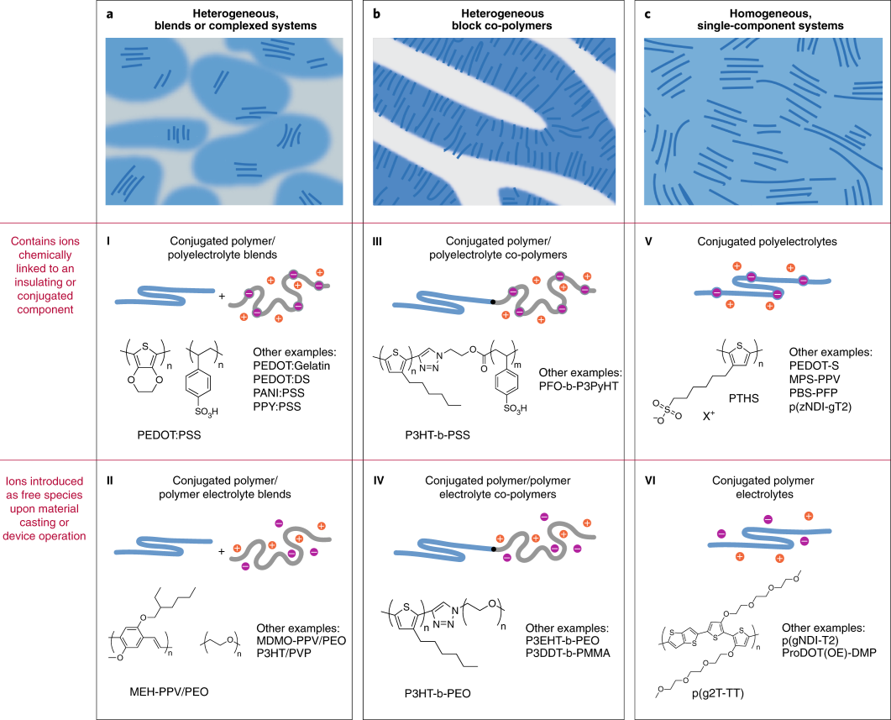
\includegraphics[width=\textwidth]{Images/OMIEC_types.png}
  \caption{\textbf{Material classes of OMIECs.} a) Heterogeneous blends of an electronically conducting conjugated polymer with (I) an ionic charge bearing polyelectrolyte or (II) an ion solvating polymer electrolyte. %These systems frequently feature impure phases and can be largely disordered on multiple length scales. 
  b) Heterogeneous block copolymers of an electronically conducting conjugated polymer with (III) an ionic charge bearing polyelectrolyte or (IV) an ion solvating polymer electrolyte. %Such block copolymers often feature more well-defined pure phases and mesoscale order—readily synthetically tunable. 
  c) Fully conjugated (V) ionic charge bearing polyelectrolytes and (VI) ion solvating polymer electrolytes. %OMIEC types I–IV produce heterogeneous morphologies with microphase segregated predominately electron conducting and ion conducting domains. As shown in the sketches in the first row, in the case of blends (I and II) this occurs in a disordered fashion, or in the case of block copolymers (III and IV) it can occur in a variety of ordered structures (lamellar phase portrayed here). All-conjugated polyelectrolytes (V) and polymer electrolytes (VI) exist as a single mixed conducting phase that may contain heterogeneous composition of ordered and amorphous domains. Conceptual sketches (grey, ionic transport component; blue, electronic transport component; orange, cations; magenta, anions) 
  Extracted from reference \cite{paulsenOrganicMixedIonic2020}.}
  \label{fig:omiectypes}
\end{figure}

\subsection{Processes in OMIECs}

\subsubsection{Ionic-electronic interactions}
The presence of electronic charge in OMIECs requires also the presence of excess ionic charge, so charge in the system remain balance. In the case of types II, IV and VI OMIECs, the so-called stabilizing electrochemical doping is achieved by the presence of mobile ions, the remaining type of OMIEC on the other hand, have this stabilizing charges fixed, they are inherently doped.

% Explanation of parts where ion-coupling (electrostatic or direct electron transfer cases) occurs, and a third case where it does not occur, not necessary here, or would it be? I think this is the main difference on what is happening in my material, compared to PEDOT:PSS. So not sure if add the graphs

The amount of coupling between electronic charge and excess ionic charge in OMIECs can be modulated with an applied bias when coupled through an electrolyte \cite{paulsenOrganicMixedIonic2020}. This is the basic principle of OECTs, and we will be further discuss in section \ref{sec:OECTs}.

\subsubsection{Electronic transport}
Electronic charge carrier density in undoped semiconductor organic species is logically low (no accessible hopping states), but in contact with an electrolyte, due to the ionic-electronic coupling as described in previous section, dopant ions would lower the activation energy of charge hopping and increase carrier mobility \cite{paulsenOrganicMixedIonic2020}. Electronic charge transport mechanisms, that can be within the length of the conjugated polymer (thermally activated hopping) or within the polymer-stacking (band-like transport) are represented in Figure \ref{fig:etrans}.
%"at extreme doping levels, increased disorder drives carrier localization, which results in a plateau or even decrease in electronic charge carrier mobility"


%"Non-conjugated radical polymers also present a thermally activated mechanism of charge transfer between pendant radical sites, though with a significant dependence on the local self-diffusion of polymer chain to bring radical sites close enough for efficient charge transfer51. This manifests as a hopping transport of electronic carriers (Fig. 2a) that is assisted via segmental motion (described below; Fig. 2g). Also in this case disorder plays a role, producing local variations in the molecular orbital energy levels and spreading orbitals in a density of radical states52."

%\begin{figure}
%  \centering
%  \includegraphics[width=\textwidth]{Images/%OMIECetransport.png}
%  \caption{Schematic representation of electronic charge transport mechanisms: a) "Thermally activated hopping transport of a relatively localized electronic charge carrier" and b) "band-like transport of a relatively delocalized electronic charge carrier". Modified from reference \cite{paulsenOrganicMixedIonic2020}.}
%  \label{fig:omiectypes}
%\end{figure}


\begin{figure}[ht]
	\centering
	\subfloat[\textbf{Thermally activated hopping}]{{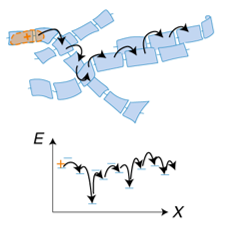
\includegraphics[width=5cm]{Images/OMIECetransport1.png} }}
	%\qquad
	\hspace{2em}
	\subfloat[\textbf{Band-like transport}]{{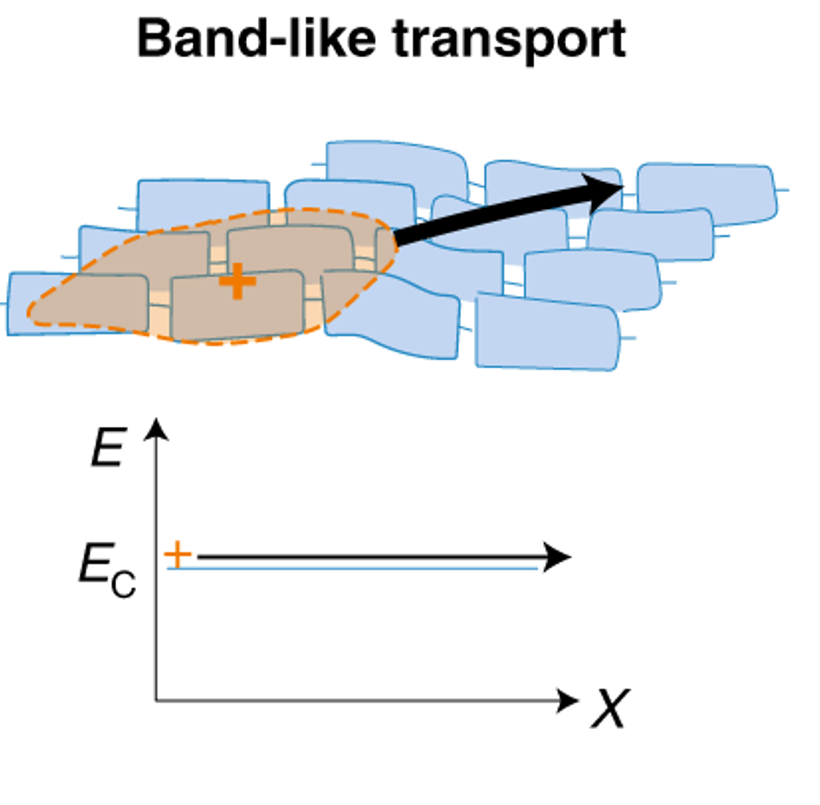
\includegraphics[width=5cm]{Images/OMIECetransport2.png} }}
	\caption{Schematic representation of electronic charge transport mechanisms: A) "Thermally activated hopping transport of a relatively localized electronic charge carrier" and B) "band-like transport of a relatively delocalized electronic charge carrier". Extracted from reference \cite{paulsenOrganicMixedIonic2020}.}a 
	\label{fig:etrans}
\end{figure}


\subsubsection{Ionic transport}
Although transport of charged anions and cations can be seen analogous to electrons and holes, they remain more complex, since they can be \textit{``multi-valent, and form pairs and larger clusters; morever, they are sensitive to solvent and solvation''} \cite{paulsenOrganicMixedIonic2020}.

Ion transport for dry OMIECs of type I, III and V are unipolar since they are fixed on a polyelectrolyte.  However, when they are in contact with an electrolyte, swelling occurs, which allows the penetration of excess ions from the electrolyte, therefore both mobile anions and cations would contribute to ion transport. 

Then two types of ionic charge transport can be differentiated: ion hopping and solvated ion vehicle transport, as described in Figure \ref{fig:itrans}A and B, respectively. In dry or minimally hydrated OMIECs only ion hopping occurs, whereas when OMIEC is in contact with solvent or liquid electrolyte, both mechanisms occur. The latter basically explains how ionic transport in OECTs (and other OMIEC-electrolyte based applications) is rather complex and needs to consider all ionic-electronic coupling, hydration and electrolyte swelling \cite{paulsenOrganicMixedIonic2020}, which will be further discuss in section \ref{sec:OECTs}.

\begin{figure}[ht]
	\centering
	\subfloat[\textbf{Ion hopping} via segmental motion\\\hspace{1em} or ion clusters]{{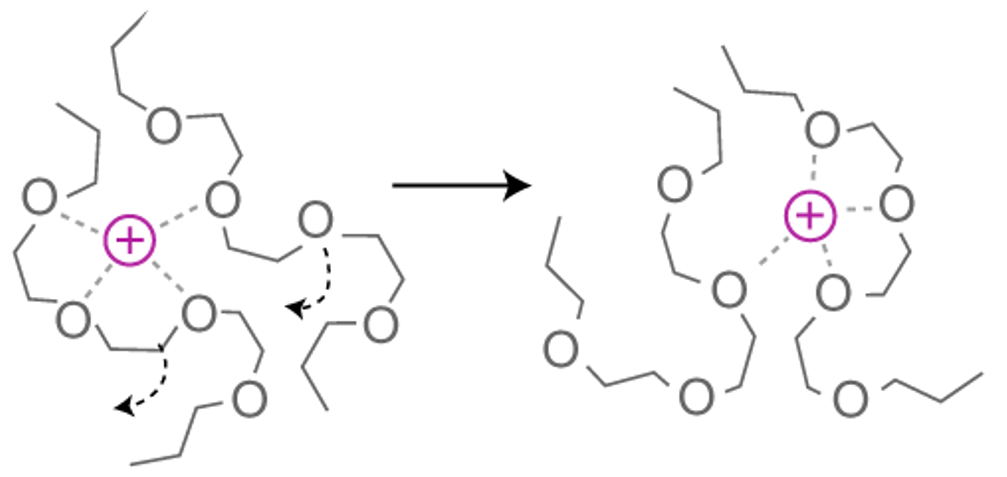
\includegraphics[width=7cm]{Images/OMIECitransport1.png} }}
	%\qquad
	\hspace{2em}
	\subfloat[\textbf{Solvated/vehicle mechanism}]{{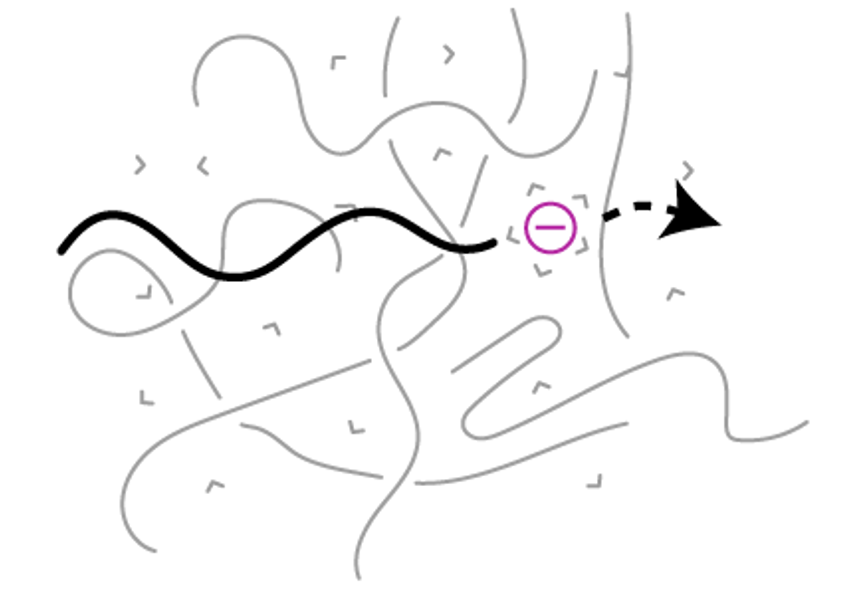
\includegraphics[width=5cm]{Images/OMIECitransport2.png} }}
	\caption{Schematic representation of ionic charge transport mechanisms: A) "Segmental motion-assisted ion hopping" and B) "solvated ion vehicle transport". Extracted from reference \cite{paulsenOrganicMixedIonic2020}.}
	\label{fig:itrans}
\end{figure}

\subsection{Electrochemical Doping}

"The electrochemical charging of OMIECs can be described as a capacitive faradaic charging process,
% there is current caused by charge transfer, other physical phenomenas such as desorption or adsorption can also lead to the aparition of current that is non faradaic reaction
meaning that the OMIEC" is p-doped (oxidized, in the language of chemists) "through an electron transfer with the contact (current collector), while ions from the electrolyte penetrate inside the channel material to compensate the charge carriers on the polymer backbone electrostatically with no change in the inserted ion's oxidation state" \cite{giovannittiEnergeticControlRedoxActive2020}

\section{Organic Electrochemical Transistors (OECTs)} \label{sec:OECTs}

Organic Electrochemical Transistors (OECTs) consists of metallic source, drain and gate electrodes, an organic conjugated polymer channel (specifically an OMIEC as described in previous sections) and an electrolyte that couples channel and gate. Devices that have received increasingly attention due to their mechanically compliance, biocompatibility, and are sensitive to biochemical modules \cite{tanMixedIonicElectronic2022}. 

%\begin{figure}[ht]
%	\centering
%	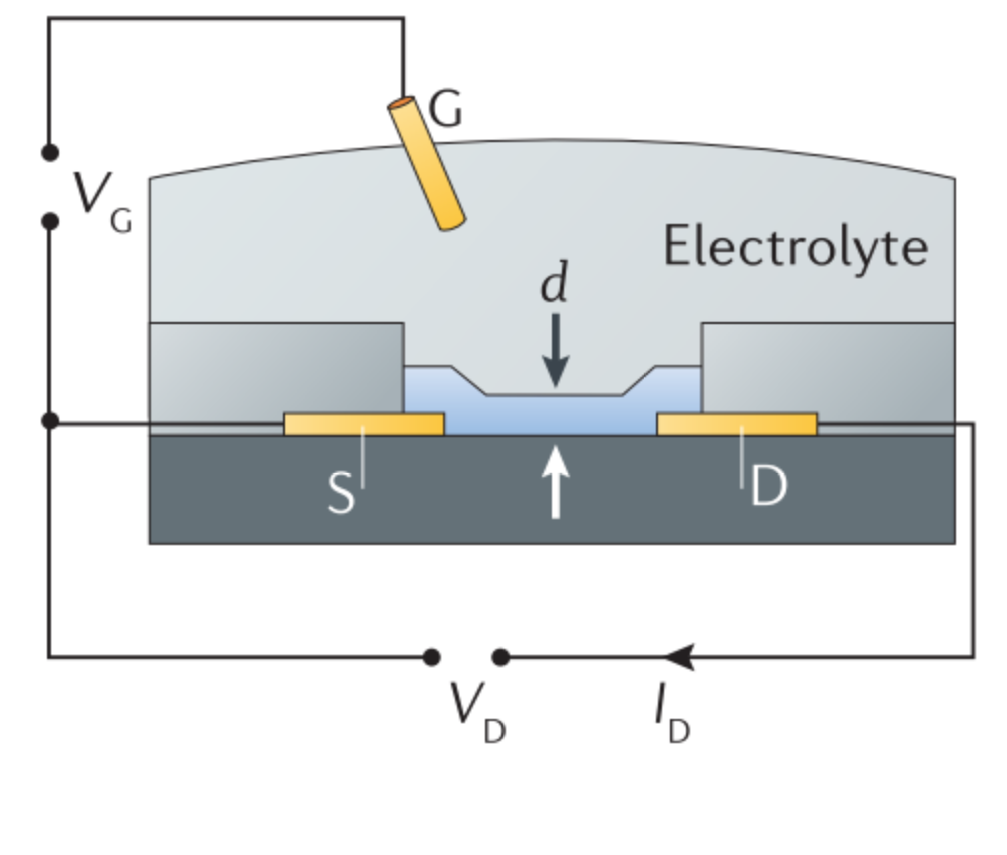
\includegraphics[height=4.5cm]{Images/structure.png}
%	\caption{Typical structure of an organic electrochemical transistor (OECT) \cite{rivnayOrganicElectrochemicalTransistors2018}.}
%	\label{fig:modes}
%\end{figure}


\subsection{Device Physics}

Although the structure of OECTs are different from conventional metal-oxide-semiconductor field-effect transistors (MOSFETs). The basic understanding of the latter can give us a clear idea of how OECTs operate. Unlike MOSFETs, OECTs are coupled with an electrolyte rather than an insulator. So, when applying a gate voltage, instead of polarizing the dipoles in the insulator, creating a field that causes accumulation of carriers at the interface of the semiconductor/insulator as it happens in a MOSFET, in an OECT, the gate voltage drives ions to penetrate the bulk of the channel, therefore accumulation of carriers will happen throughout the whole volume of the OMIEC film. This explains the large gate-channel capacitance in these devices compared to MOSFETs, and why drain-source current takes into account a volumetric capacitance \cite{friedleinDevicePhysicsOrganic2018}.


\begin{figure}
  \centering
  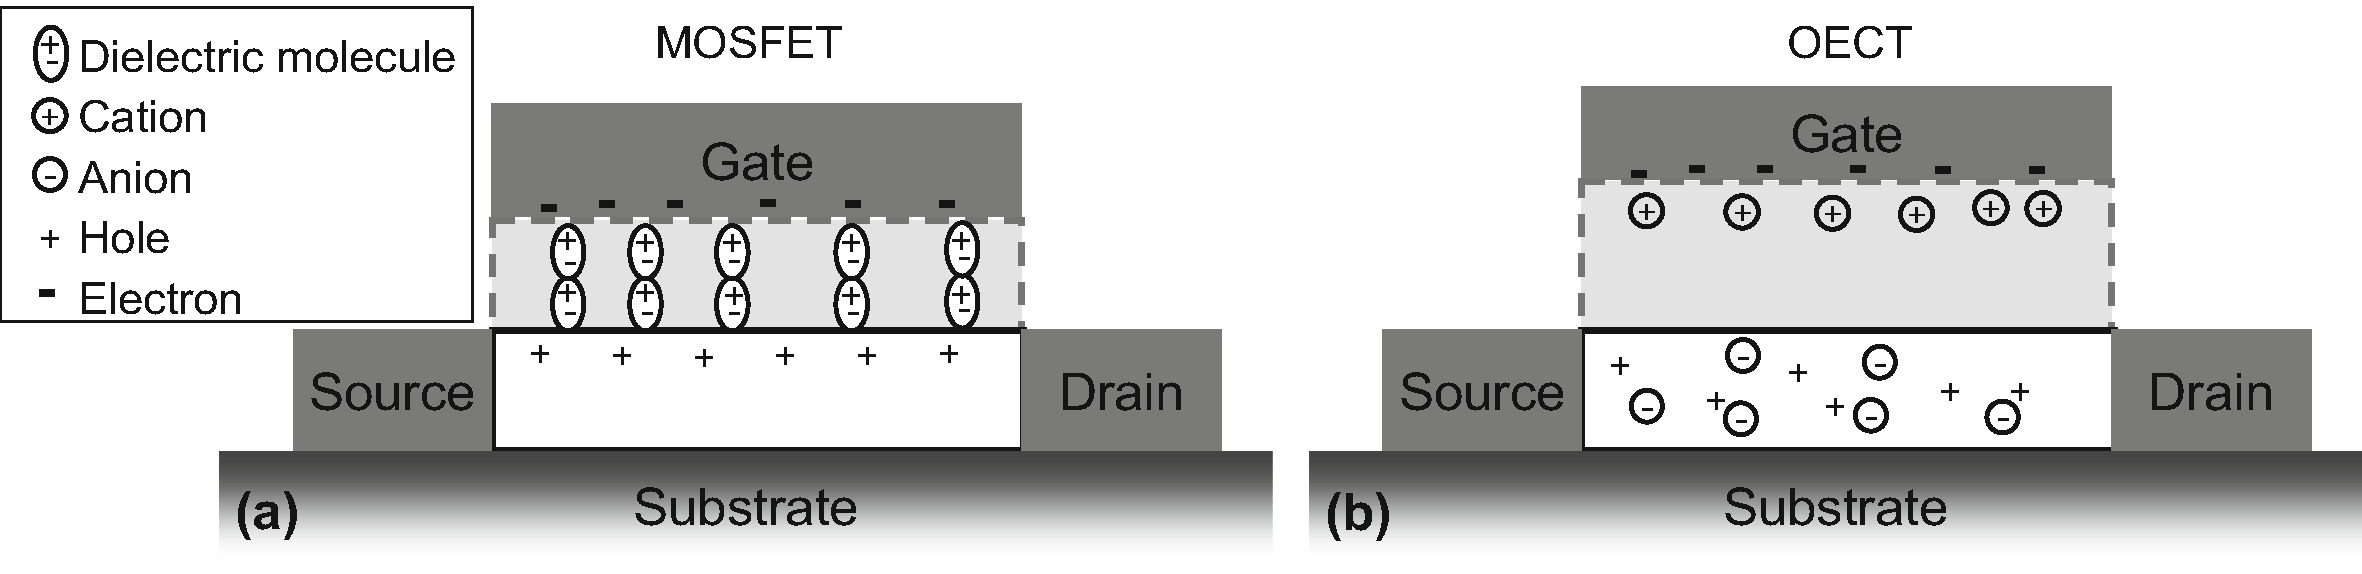
\includegraphics[width=\textwidth]{Images/MOSFETvsOECTs.jpg}
  \caption{Comparison of p-type A) MOSFET and B) OECT. Where the light-gray region represents an insulator and a electrolyte, respectively. Extracted from reference  \cite{friedleinDevicePhysicsOrganic2018}}
  \label{fig:vsMOS}
\end{figure}

Bernard et al. implemented a model based on a p-type depletion-mode OECT (based on PEDOT:PSS since it is widely fabricated and investigated, further discussion in the following section). The model divides the behavior of the OECT into an electronic (source-channel-gate structure) and an ionic circuit (gate-electrolyte-channel structure). The electronic circuit is treated as a \textit{variable} resistor therefore it is modeled using Ohm's law, its variability lies on the fact that upon the application of a positive gate voltage, de-doping of the semiconductor occurs: analogous to the compensation doping of Silicon, cations from the electrolyte penetrate the polymer, compensating one acceptor. Meanwhile, the ionic circuit is consists of a resistor that represents the flow of ions in the electrolyte, in series with a capacitor, representing the storage of ions in the channel as represented in Figure \ref{fig:bernard}C) \cite{rivnayOrganicElectrochemicalTransistors2018}\cite{bernardsSteadyStateTransientBehavior2007}. 

\begin{figure}[ht]
	\centering
	\subfloat[]{{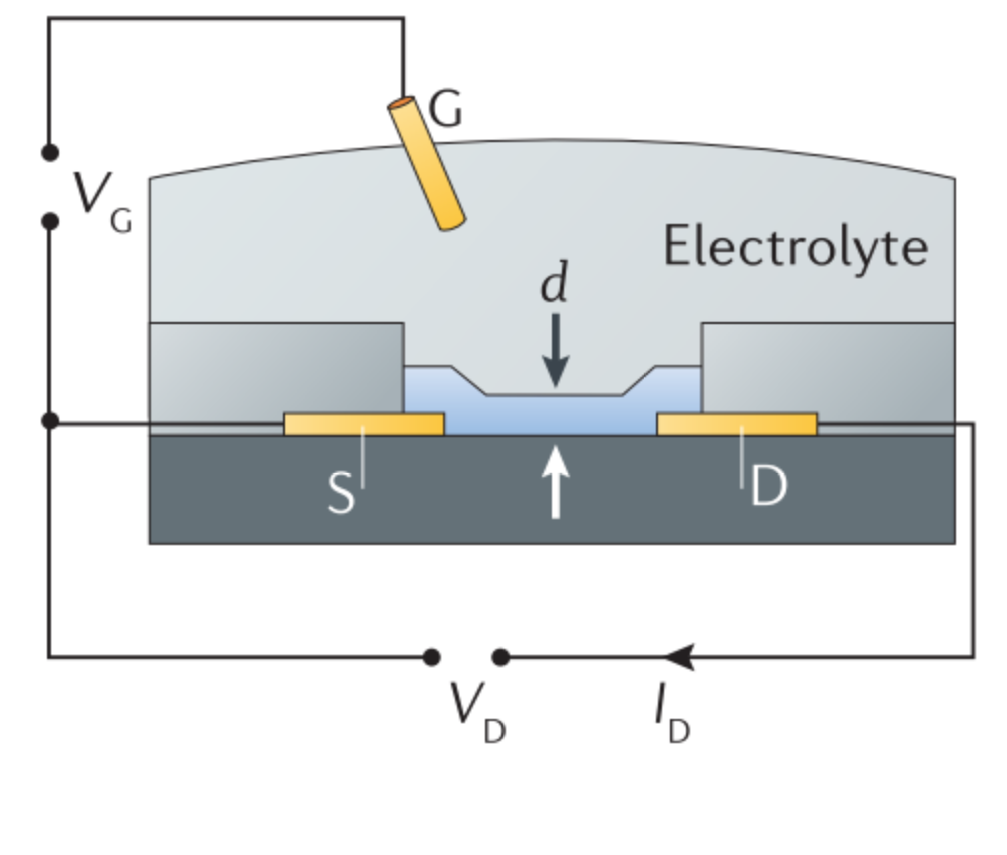
\includegraphics[width=4.5cm]{Images/structure.png} }}
	%\qquad
	\subfloat[]{{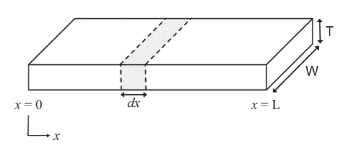
\includegraphics[height=1.5cm]{Images/film_model.png} }}
	\subfloat[]{{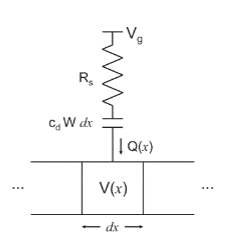
\includegraphics[height=4.5cm]{Images/circuit_model.png} }}
	\caption{A) Typical structure of an organic electrochemical transistor (OECT). Extracted from reference \cite{rivnayOrganicElectrochemicalTransistors2018}. Representation of device model, B) OMIEC film with source and drain located at x=0 and x=L, respectively, C) Ionic circuit charge (Q) is coupled to the voltage in the electronic circuit. Images extracted from reference \cite{bernardsSteadyStateTransientBehavior2007}.}
	\label{fig:bernard}
\end{figure}


\subsection{Operation Modes}

Analogous to conventional MOSFETs, depending on whether the device needs a gate potential to turn it ON, it will describe two operation modes, in the case of OECTs: depletion and accumulation. Specifically in OECTs, these modes have a strict relationship to the channel material, if it is inherently conductive or semiconducting.

\begin{figure}[ht]
	\centering
	\subfloat[]{{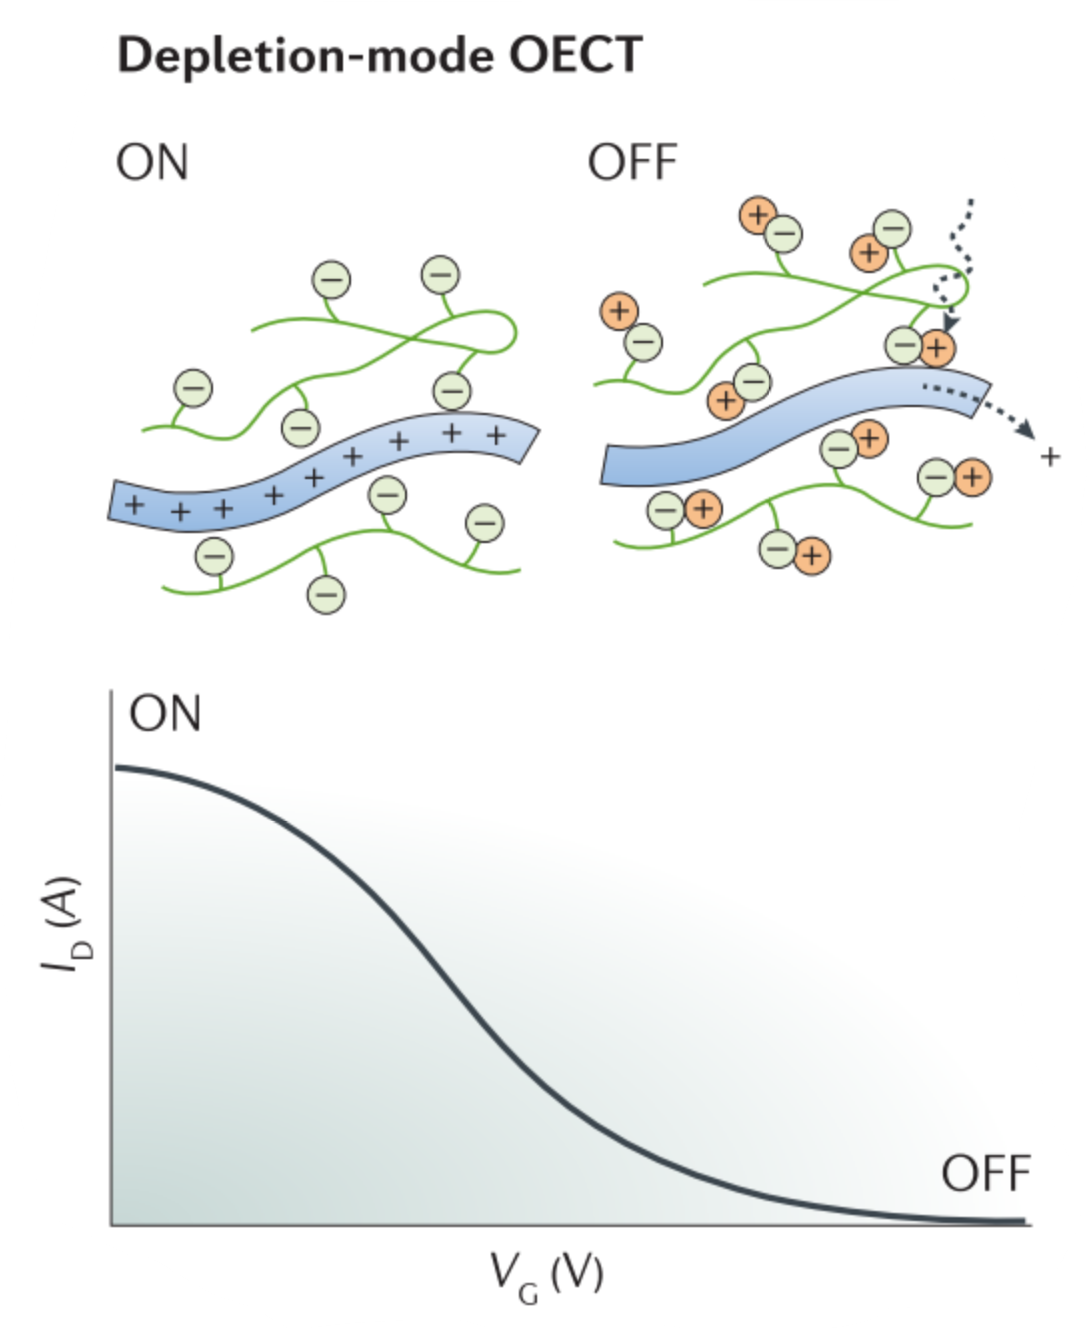
\includegraphics[height=7cm]{Images/depletion.png} }}
	\subfloat[]{{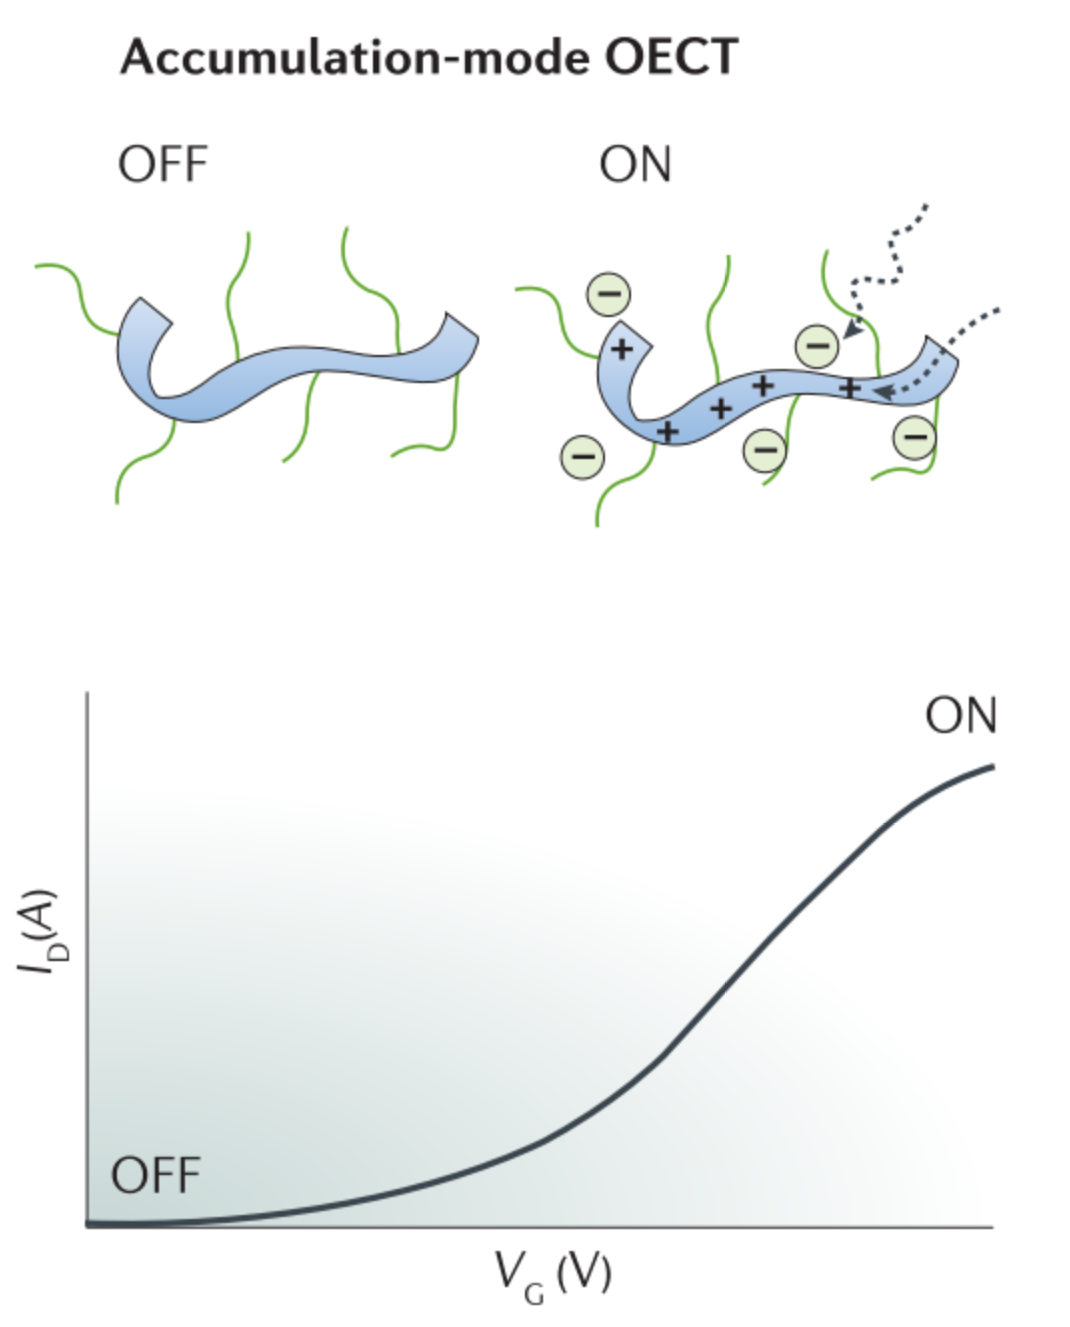
\includegraphics[height=7cm]{Images/accumulation.png} }}
	\caption{(A) Transfer curve showing depletion-mode operation of a p-type OECT with a conducting polymer channel. (B) Transfer curve showing accumulation-mode operation of a p-type OECT with a semiconducting polymer channel. Images extracted from reference \cite{rivnayOrganicElectrochemicalTransistors2018}.}
	\label{fig:modes}
\end{figure}

As seen in Figure \ref{fig:modes}A) and B), the polymer can be conductive or semiconducting. In the first scenario, the OMIEC already possesses anions which have had induced charges within its backbone, therefore it needs the injection of cations to counteract this effect, hence turn OFF the device. The opposite scenario is shown for a semiconducting polymer channel, an OECT will normally be OFF without the application of a gate voltage.

\subsubsection{Standard material for depletion-mode OECTs}

%\subsection{Engineering of semiconducting polymers}
Poly(3,4-ethylenedioxythiophene) poly(styrene-sulfonate) (PEDOT:PSS) is a ``degenerately doped''\cite{bernardsSteadyStateTransientBehavior2007} polymer that is widely used in multiple applications in organic electronics. Classified as type I OMIEC, as seen in Figure \ref{fig:omiectypes}. It is a blend between a conjugated polymer (PEDOT) and a polyelectrolyte (PSS), the latter posseses chemically linked ions and serves as a polymeric acid template to allow dispersable suspensions \cite{paulsenOrganicMixedIonic2020}.

Due to its commercial availability, operational stability, and relatively high performance, PEDOT:PSS became a standard material for p-type OECTs. Its main drawback lays in its depletion-mode operation, since, as explained in the previous section, requires power to turn off. 

With the aim of minimizing power consumption, there is a special interest to design semiconducting polymers that would allow accumulation-mode devices with high performance \cite{nielsenMolecularDesignSemiconducting2016}\cite{tanOrganicMixedIonic2022}\cite{inalBenchmarkingOrganicMixed2017}\cite{keeneEnhancementModePEDOTPSS2020}. This type of devices has the advantage of dissipating less static power when the device is not operated, due to low OFF current%, which must be minimized as much as possible
\cite{giovannittiEnergeticControlRedoxActive2020}.

\subsubsection{Prospective materials for accumulation-mode OECTs}

Nielsen et al. reported a series of semiconducting polymers with Triethylene glycol (TEG) side chains designed to compare their performance as accumulation-mode OECTs. Among the five thiophene- and benzodithiophene-based polymers, they found out that the TEGylated bithiophene unit (g2T-T) shown the highest performance, even highest transconductance over PEDOT:PSS \cite{nielsenMolecularDesignSemiconducting2016}. Since its backbone design warrant reversibility during electrochemical redox reactions and good electronic transport, meanwhile the EG side chains enable its stability in aqueous electrolytes and efficient transport of ionic and electronic charge carrier \cite{moiaDesignEvaluationConjugated2019}. 
%% moia es el unico que tiene un dibujo distinto de pg3t

Moser et al. studied the impact of the length of the EG side chain of this thiophene backbone on the performance of OECTs. They reported that reducing chain length would maximize the capacitance, but the increase of length would enhance ion-polymer interaction. Finally, they suggested an optimum length of 3 monomers in side chains over 2, 4 and 6 monomers, demonstrating that an OECT with 3-(2-(2-(2-methoxyethoxy)ethoxy)ethoxy)thiophene p(g3T2-T), as seen in Figure \ref{fig:pg3t}, has higher transconductance, and a turn-on voltage close to zero compared to other thiophene-based species, additionaly the absence of extensive pre- and postprocessing to optimize polymer stability and electrochemical performance in aqueous media and the possibility of an accumulation-mode OECT with low operation voltages put it on top of PEDOT:PSS \cite{moserEthyleneGlycolBasedSide2020}.

%Seria chevere tener un grafico de como thiophene publications empezaron a crecer.
%Thiophene is a planar conjugated ring structure consists of six delocalized pi-electrons. The aromatic nature arises from the four $\pi$-electrons and one unshared lone pair of electrons of the oxygen as six delocalized $\pi$-electrons. It folow Hucke´s rule. Hence it is aromatic compound.

%Homogeneous single phase OMIECs (types V and VI) display larger magnitudes of ionic–electronic coupling and larger values of volumetric capacitance than biphasic OMIECs (types I–IV) \cite{paulsenOrganicMixedIonic2020}. 

Under the classification shown in Figure \ref{fig:omiectypes}, p(g3T2-T) can be identified as a type VI OMIEC that comprises a conjugated polymer with ions introduced as \textbf{free species} wheareas PEDOT:PSS' ions are \textbf{chemically linked} to the polyelectrode (PSS) and blended to the conjugated polymer (PEDOT). This structural characteristic make p(g3T2-T) display larger magnitudes of ionic-electronic coupling but at the same time will be important for understanding the challenges on having a stable OECT with our material and will be bring back in Section \ref{subsec:req}.


\begin{figure}
  \centering
  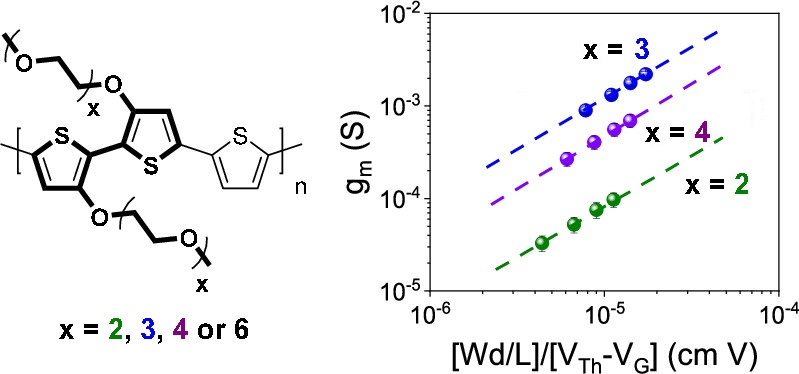
\includegraphics[width=5cm]{Images/pg3t+perf.jpeg}
  \caption{(Left) Chemical structure of the repeat units for p(gxT2-T). (Right) Transconductance vs channel geometry and operating parameters of p(gxT2-T) for x = 2, 3 and 4. Extracted from reference \cite{moserEthyleneGlycolBasedSide2020}}
  \label{fig:pg3t}
\end{figure}


\subsection{Important Figures of Merit}

\subsubsection{Transconductance}

\subsubsection{$\mu$C* product}


The modulation of the degreee of electrochemical doping in OECTs with an applied biased, will manifest a potential-dependent capacitance (C). Homogeneous single phase OMIECs (type V and VI) display larger magnitudes of ionic-electronic coupling and larger values of volumetric capacitance than biphasic OMIECs such as PEDOT:PSS \cite{inalBenchmarkingOrganicMixed2017}
% found in Paulsen \cite{paulsenOrganicMixedIonic2020}
%actually from reference 44, benchmarking omiecs for transistors

\subsubsection{Threshold voltage}

An approach to shift the operating voltage range for PEDOT:PSS OECTs to lower the channel current, leading to reduced power consumption, is to tune the threshold voltage by de-doping PEDOT:PSS using commercially available amine-based molecular de-dopants \cite{keeneEnhancementModePEDOTPSS2020}. Tan et al., on the other hand, explored a different approach, rather than modifying the doping level of the channel, they tuned the doping level of the gate to shift the threshold voltage. They used p(g3T2-T) and obtained a 400mV change with 60\% mol ratio of 2,3,5,6-Tetrafluoro-7,7,8,8-tetracyanoquinodimethane (F4TCNQ) dopant. The advantage over this approach is i) protecting the material from oxidation, since the Fermi level in brought towards the highest occupied molecular orbital (HOMO), and ii) no interference with the channel which helps to leave the transconductance unaffected \cite{tanTuningOrganicElectrochemical2022}.


{\subsection{Requirements to Avoid Undesirable Side Reactions}}
\label{subsec:req}

Achieving effective charge transfer between the analyte and OMIEC requires appropriate alignment of the electrochemical potential of electrons on the OMIEC electrode and the redox specie. Failure to do so may result in the subsequent transfer of charges to other redox-active sinks in the environment, leading to undesirable side reactions and products that may interfere with the OMIEC’s operation. Electrons flow from a region of higher to lower electrochemical potential. Hence, achieving electron transfer from redox-active species to the OMIEC requires the latter to have a deep LUMO (high electron affinity) \cite{tanMixedIonicElectronic2022} %paper

Capacitive fading upon cycling

\subsubsection{Water uptake}

Savva et al. study the influence of water on the performance of OECT, the water uptake of conjugated polymer films led to 10-13\% mass increase under non biased conditions. As the concentration of water decrease (NaCl$_{aq}$ 10 mM, 100mM, 1M, and 6M) ionic charging is faster regardless of the doping pulse, however the fastest ionic charging is achieved at NaCl$_{aq}$ 1 M. The injection/drift of ions is also affected by the ion-counterion attractive forces which delays the ion injection from the electrolyte, opposing their drift into the polymer (NaCl$_{aq}$ 6 M hinders the drift of anions) affecting the response time. \cite{savvaInfluenceWaterPerformance2019}

\subsubsection{Oxygen Reduction Reaction (ORR)}

With the aim of developing accumulation-mode OECTs, the engineering of new OMIECs were introduced as commented in previous sections. Normally, this polymer backbones have low ionization potential (IPs) which lead to another side effect issue that little attention has been paid: non capacitive faradaic rections in ambient: electron-transfer reaction from the OMIEC to molecular oxygen described as oxygen reduction reaction (ORR)

% Remember 
% Thermodynamically favored processes or reactions are those that involve both a decrease in the internal energy of the components (ΔH° < 0) and an increase in entropy of the components (ΔS° > 0). These processes are necessarily “thermodynamically favored” (ΔG° < 0) or negative. ΔG° = ΔH°-TΔS°
% Catalyst help to reduce the activation energy required for a reaction

The ORR yields either H$_{2}$O$_{2}$ or water (H$_{2}$O) as well as charging (oxidation) of the OMIEC that acts as the catalyst. The first shows a free energy difference that is endergonic for OMIECs with IPs \> 4.9eV and hence prevent the OMIEC from undergoing ORR that form H$_{2}$O$_{2}$. To prevent the ORR in ambient conditions, OMIECs based on donor-acceptor copolymer (Type III or IV) that have large IPs to shift
\cite{giovannittiEnergeticControlRedoxActive2020}
% Actually this material does not avoid this, we need to take into account this interaction.

\subsection{Building Block for neuromorphic and bioelectronic applications}



%%% Local Variables: 
%%% mode: latex
%%% TeX-master: "thesis"
%%% End: 
